


\begin{figure}[ht]
    \centering
    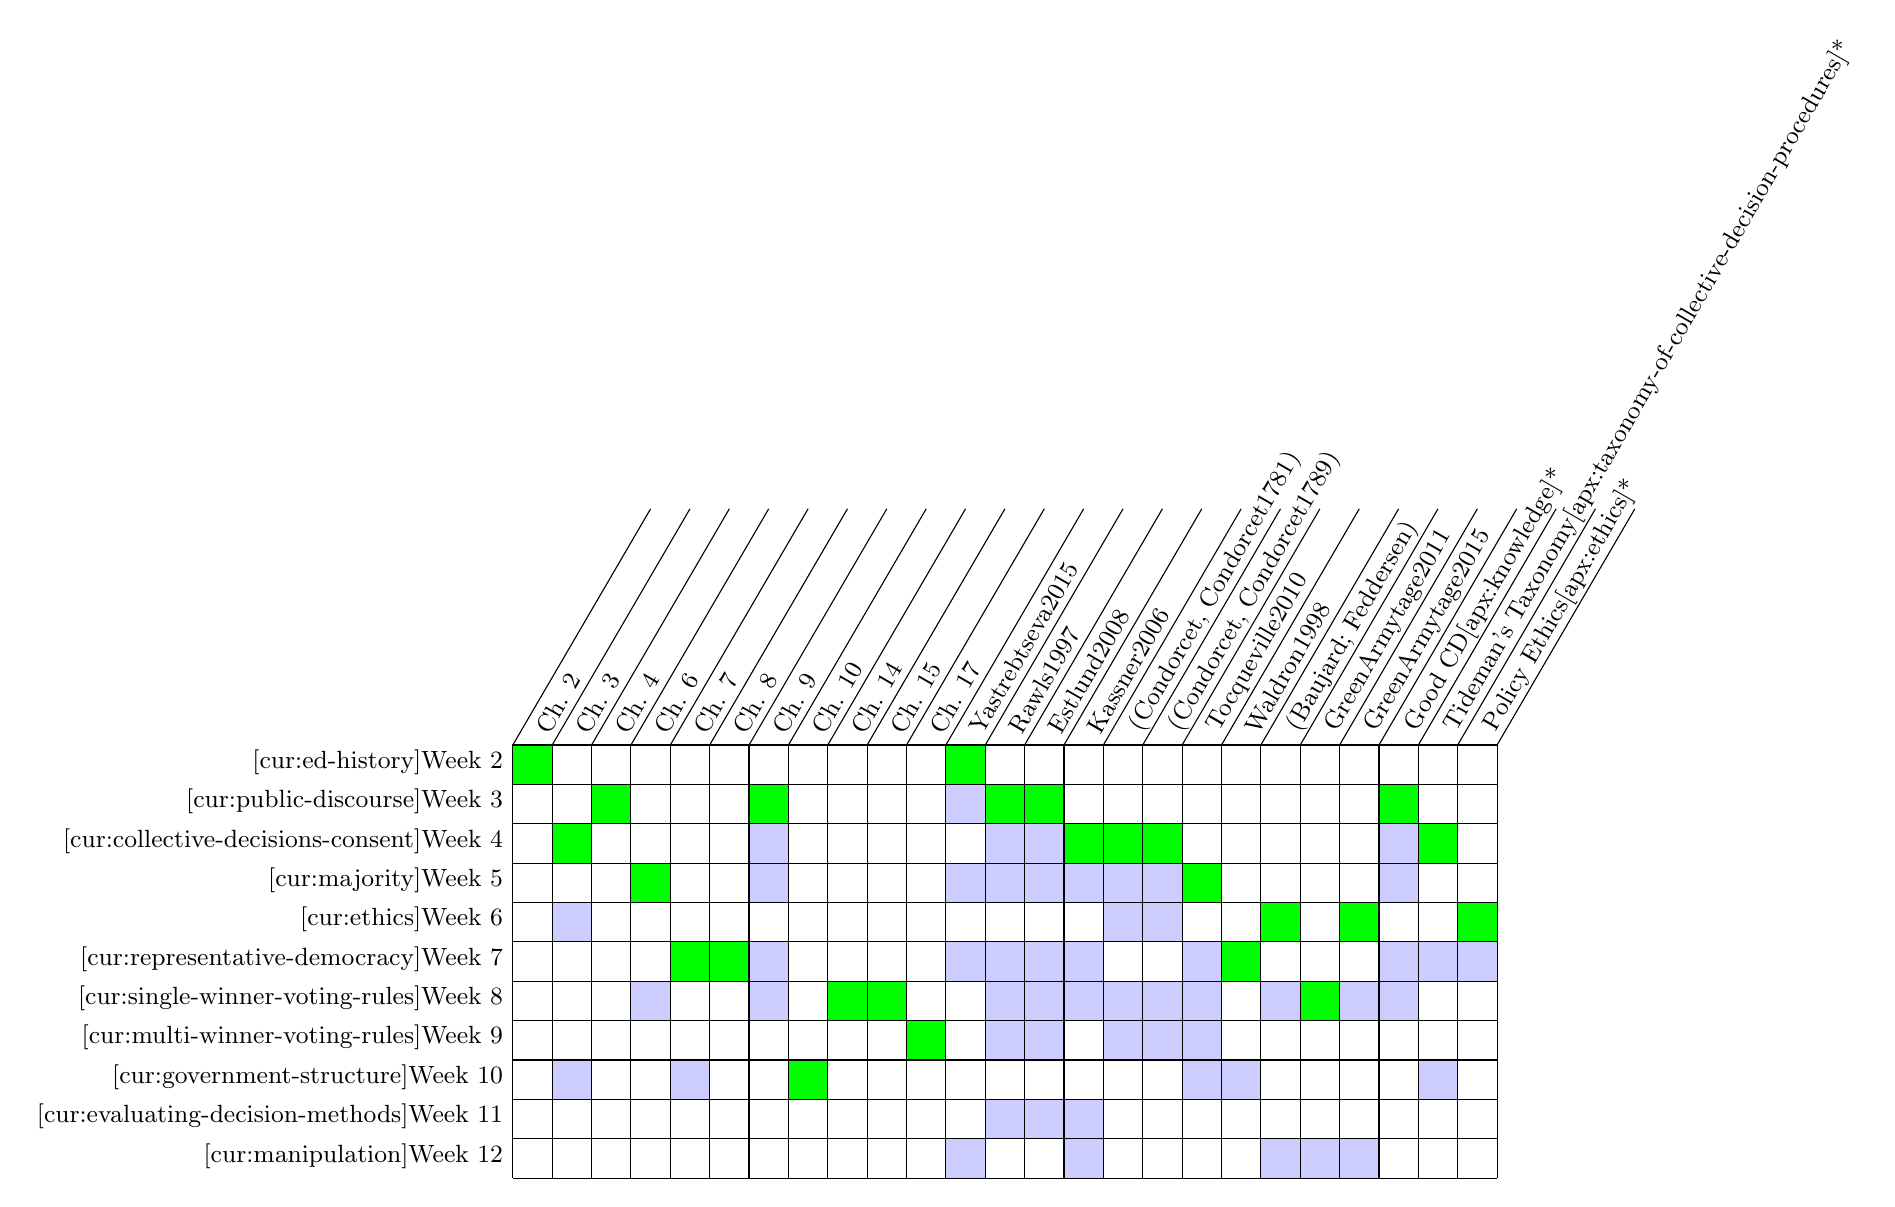
\begin{tikzpicture}[
        %sibling distance=10em,
        font=\small,
        ]
    \foreach \x[count=\xi from 0] in {
        2, % Ch. 2
        4,
        3,
        5,
        7,
        7,
        3,
        10,
        8,
        8,
        9,
        2,
        3,
        3,
        4,
        4,
        4,
        5,
        7,
        6, % Baujard and Feddersen
        8, % Condorcet-Hare
        6, % Green-Armytage,
        3, % Good CD/knowledge
        4, % Taxonomy
        6 % Ethics
    }
    {
        \draw [fill=green] (\xi/2,1-\x/2) rectangle ++(0.5,-0.5);
    }
    \foreach \x / \y in {
        1/6, 1/10,
        3/8,
        4/10,
        6/4, 6/5, 6/7, 6/8,
        11/3, 11/5, 11/7, 11/12,
        12/4, 12/5, 12/7, 12/11, 12/8, 12/9,
        13/4, 13/5, 13/7, 13/11, 13/8, 13/9,
        14/5, 14/7, 14/11, 14/8, 14/12,
        15/5, 15/6, 15/8, 15/9,
        16/5, 16/6, 16/8, 16/9,
        17/7, 17/8, 17/9, 17/10,
        18/10,
        19/8, 19/12,
        20/12,
        21/8, 21/12,
        22/4, 22/5, 22/7, 22/8, % Good CD
        23/7, 23/10,
        24/7
    }
    {
        \draw [fill=blue!20] (\x/2,1-\y/2) rectangle ++(0.5,-0.5);
    }
    \foreach \x[count=\xi] in {
        Ch. 2,
        Ch. 3,
        Ch. 4,
        Ch. 6,
        Ch. 7,
        Ch. 8,
        Ch. 9,
        Ch. 10,
        Ch. 14,
        Ch. 15,
        Ch. 17,
        \autocite{Yastrebtseva2015},
        \autocite{Rawls1997},
        \autocite{Estlund2008},
        \autocite{Kassner2006},
        {(Condorcet, \citeyear{Condorcet1781})},
        {(Condorcet, \citeyear{Condorcet1789})},
        \autocite{Tocqueville2010},
        \autocite{Waldron1998},
        {(Baujard; Feddersen)},
        \autocite{GreenArmytage2011},
        \autocite{GreenArmytage2015},
        Good CD\hyperref[apx:knowledge]{*},
        Tideman's Taxonomy\hyperref[apx:taxonomy-of-collective-decision-procedures]{*},
        Policy Ethics\hyperref[apx:ethics]{*},
        {}
    }
    {
        \node at (0.5*\xi-0.35,0) [anchor=south west] {\rotatebox{60}{\x}};
        \draw (0.5*\xi-0.5,0) -- ++(1.75,3);
        \draw (0.5*\xi-0.5,0) -- ++(0,-12/2+0.5);
    }

    \draw (0,0) -- (12.5,0);
    \foreach \x[count=\xi] in {
        \hyperref[cur:ed-history]{Week 2},
        \hyperref[cur:public-discourse]{Week 3},
        \hyperref[cur:collective-decisions-consent]{Week 4},
        \hyperref[cur:majority]{Week 5},
        \hyperref[cur:ethics]{Week 6},
        \hyperref[cur:representative-democracy]{Week 7},
        \hyperref[cur:single-winner-voting-rules]{Week 8},
        \hyperref[cur:multi-winner-voting-rules]{Week 9},
        \hyperref[cur:government-structure]{Week 10},
        \hyperref[cur:evaluating-decision-methods]{Week 11},
        \hyperref[cur:manipulation]{Week 12}
    }
    {
        \node at (0,-0.5*\xi) [anchor=south east] {\x};
        \draw (0,-0.5*\xi) -- (12.5,-0.5*\xi);
    }

    \end{tikzpicture}
    \caption{\label{fig:resources}Resources and concepts introduced and later discussed.}
\end{figure}